\chapter*{Tác giả}
\addcontentsline{toc}{chapter}{Tác giả}
\setheader{Tác giả}

%% Print the full name of the author.
\begin{wrapfigure}{l}{1.05in}
\vspace{-0.19in}
{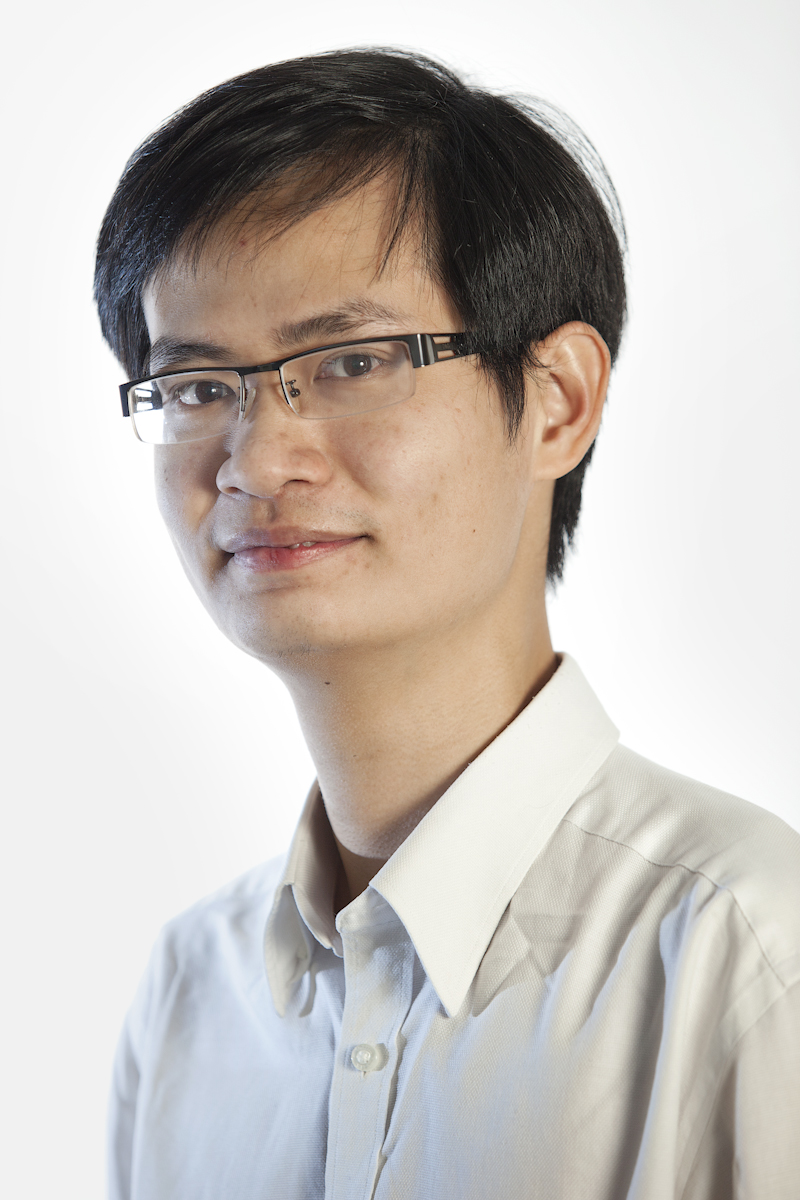
\includegraphics[width=1.25in,height=1.35in,clip,keepaspectratio]{preface/figure/img.jpg}}
\vspace{-0.19in}
\end{wrapfigure}
\textbf{Phạm Quốc Cường} sinh ra và lớn lên tại tỉnh Tiền \mbox{Giang}. Cường nhận bằng Đại học chuyên ngành Khoa học và Kỹ thuật Máy tính tại Trường Đại học Bách Khoa - Đại học Quốc gia TP.HCM năm 2007. Sau khi tốt nghiệp đại học, Cường công tác tại Khoa Khoa học và Kỹ thuật Máy tính với vai trò giảng viên. Năm 2009, Cường nhận bằng Thạc sĩ chuyên ngành Khoa học Máy tính tại cùng trường. Tháng 4 năm 2011, Cường chuyển sang phòng thí nghiệm Kỹ thuật Máy tính, Trường Đại học Công nghệ Delft, Hà Lan (the Computer Engineering lab, Delft University of Technology, the Netherlands) làm nghiên cứu sinh dưới sự hướng dẫn của GS.TS Koen Bertels, trưởng phòng thí nghiệm, và TS Zaid Al-Ars. Tháng 4 năm 2015, Cường nhận bằng Tiến sĩ của Trường Đại học Công nghệ Delft, Hà Lan và quay trở lại Khoa Khoa học và Kỹ thuật Máy tính Trường Đại học Bách Khoa - Đại học Quốc Gia TP.HCM. Hiện tại, TS Cường là giảng viên thuộc Bộ môn Kỹ thuật Máy tính, Khoa Khoa học và Kỹ thuật Máy tính, Trường Đại học Bách Khoa - Đại học Quốc gia TP.HCM. Các hướng nghiên cứu chính của TS Cường là: reconfigurable computing, hybrid interconnect, multi/many cores architecture, hardware/software co-design.